\subsection{A better Complexity Analysis of the original algorithm}

In the article \cite{art:2DGrid}, Andris Ambainis give us a quantum algorithm to recognize
the belonging of a $n$ length bit string in $\Dyck{k, n}$ using
$O(\sqrt{n}(\log_2(n))^{0.5k})$ quantum queries. But the quantum query complexity for $k=1$ is not as good as a
Grover's search which is sufficient. More precisely, for $k=1$ the algorithm is
searching for a minimal $\pm 2$ string in $1x0$ but every minimal $\pm 2$ string
is of size $2$. So the logarithmic search of the upper bound on the size of the
minimal $\pm 2$ string is no more useful and the algorithm can be summarized to
applying a Grover search for 2 consecutive 0 or two consecutive 1. This lower the quantum
query complexity of the initial case of the function to $O(\sqrt{n})$ instead of $O(\sqrt{n\log_2(n)})$.
This give us this following algorithm for \FA{k}.

\begin{algorithm}
    \caption{\FA{k}(l,r,s)}\label{alg:FA_prim}
    \begin{algorithmic}
        \Require $0 \leq l < r$ and $s \subseteq \{1,-1\}$
        \If{$k > 2$}
        \State \textbf{Find} $d$ in $\{2^{\lceil \log_2(k)\rceil }, 2^{\lceil \log_2(k)+1\rceil },\ldots,2^{\lceil \log_2(r-l)\rceil }\}$
        such that \\
        \hspace*{1cm} $v_d \gets $ \FFL{k}$(l,r,d,s)$ is \textbf{not} \Null
        \State \textbf{return} $v_d$ or \Null \ if none
        \Else
        \State \textbf{Find} $t$ in $\{l, l+1, \dots, r\}$ such that \\
        \hspace*{1cm} $v_t \gets$ \FALM{2}$(l,r,t,2,s)$ is \textbf{not} \Null
        \State \textbf{return} $v_t$ of \Null \ if none
        \EndIf
    \end{algorithmic}
\end{algorithm}

The same improvement can be done on \FFP{k} because if $k = 2$ the logarithmic
search is useless. So \FFP{k} can be redefined as in \textsc{Algorithm} \autoref{alg:ffp_better}.
For $k=2$, the complexity is lowered from $O(\sqrt{\log_2(l-r)})$ to $O(1)$.

\begin{algorithm}
    \caption{$\FFP{k}(l,r,t,s)$}\label{alg:ffp_better}
    \begin{algorithmic}
        \Require $0\leq l<r$, $l \leq t \leq r$ and $s \subseteq \{1, -1\}$
        \If{$k>2$}
        \State \textbf{Find} $d$ in $\{2^{\lceil \log_2(k)\rceil }, 2^{\lceil \log_2(k)+1\rceil },\ldots,2^{\lceil \log_2(r-l)\rceil }\}$
        such that \\
        \hspace*{1cm} $v_d \gets $ \FALM{k}$(l,r,t,d,s)$ is \textbf{not} \Null
        \State \textbf{return} $v_d$ or \Null \ if none
        \Else
        \ $v \gets $ \FALM{k}$(l,r,t,2,s)$ is \textbf{not} \Null
        \State \textbf{return} $v_d$ or \Null \ if none
        \EndIf
    \end{algorithmic}
\end{algorithm}

This small improvements on the initial cases will improve the global
quantum query complexity of each subroutine and finally the quantum
query complexity for \Dyck{k,n}.

\newpage

\begin{theorem}{\textbf{\Dyck{k,n}'s algorithm correctness}} \label{th:subroutine_correctness}
    The new definition of \FA{} and \FFP{} does not change the behavior the original algorithm
    as other subroutines (\autoref{annex:complete_subroutine_dyck_kn}) stay unchanged.
\end{theorem}

\begin{tproof}
    The behavior of the \Dyck{k,n} algorithm with the new subroutines is the same than the older
    one as \FA{} (resp. \FF{}) has the same sub-behavior on every entry with its
    older definition.
\end{tproof}

\begin{theorem}{\textbf{\Dyck{k,n}'s Subroutines complexity}} \label{th:subroutine_complexity}
    The subroutines' quantum query complexity for $k$ are the following.
    \begin{enumerate}
        \item $Q$(\Dyck{k,n}) = $O\left(\sqrt{n}(\log_2(n))^{0.5(k-1)}\right)$ \ for $k \geq 1$
        \item $Q$(\FA{k+1}$(l,r,s)$) = $O\left(\sqrt{r-l}(\log_2(r-l))^{0.5(k-1)}\right)$ \ for $k \geq 1$
        \item $Q$(\FFL{k+1}$(l,r,d,s)$) = $O\left(\sqrt{r-l}(\log_2(r-l))^{0.5(k-2)}\right)$ \ for $k \geq 2$
        \item $Q$(\FALM{k+1}$(l, r, t, d, s)$) = $\left\{
                  \begin{array}{ll}
                      O\left(\sqrt{d}(\log_2(d))^{0.5(k-2)}\right) & \textrm{for} \ k \geq 2 \\
                      O(1)                                         & \textrm{for} \  k = 1
                  \end{array}
                  \right.$
        \item $Q$(\FF{k}$(l,r,s, left)$) = $O\left(\sqrt{r-l}(\log_2(r-l))^{0.5(k-2)}\right)$ \ for $k \geq 2$
        \item $Q$(\FFP{k}$(l,r,t,s)$) = $\left\{ \begin{array}{ll}
                      O\left(\sqrt{r-l}(\log_2(r-l))^{0.5(k-2)}\right) & \textrm{for} \ k \geq 3 \\
                      O(1)                                             & \textrm{for} \ k = 2
                  \end{array}
                  \right.$
    \end{enumerate}
\end{theorem}

\begin{tproof}
    The idea is that only the $O\left(\sqrt{n}\right)$ comes from the initial cases for $k = 1$ and
    for each of the $k-1$ level of the recursion, the quantum query complexity is increased by
    a $O\left(\sqrt{\log_2(n)}\right)$ factor. The $O\left(\sqrt{\log_2(n)}\right)$ factor
    is proven by Andris Ambainis' team in \cite{art:2DGrid} while the $O\left(\sqrt{n}\right)$
    for $k = 1$ comes from the new version of \FA{k} (\textsc{Algorithm} \autoref{alg:ffp_better}).
    The complete proof for the theorem is given in \autoref{proof:complexity_dyckkn}.
\end{tproof}

Unfortunately, the improvements done on the initial cases of some of the subroutines are not sufficient
to get a significant improvement for the quantum query complexity of \Dyck{k,n} algorithm. In order to
improve more the query complexity, an other algorithm using a different strategy should be found.

\subsection{A new algorithm for \Dyck{2,n}}

First, we would like to find an algorithm with a quantum query complexity near to match the lower bound,
$\exists c > 1$ such that $Q\left(\Dyck{k,n}\right)=\Omega\left(\sqrt{n}c^k\right)$, describes by Andris
Ambainis' team in \cite{art:2DGrid}. So the searched algorithm must have a quantum query
complexity of $O\left(\sqrt{n}\right)$.

For $k=1$, the query complexity comes only from a call to Grover's search
because rejecting is easily by finding a 00 or a 11 substrings inside the entry. For $k=2$
it no more possible as the substrings that reject are of the form 00(10)*0 or of the form 11(01)*1. It
implies that the number of calls to Grover's search in the naive approach is in $O\left(n\right)$ so the
quantum query complexity finally becomes $O\left(n\sqrt{n}\right)$. In order to keep it in
$O\left(\sqrt{n}\right)$, the algorithm must do a constant number of calls to Grover's search.

For that, we define a new alphabet that can express every even length binary
strings and that have convenient property for a Grover's search. Let
$\mathcal{A} = \{a, b, c, d\}$ the alphabet where $a$ corresponds to 00, $b$ to 11, $c$
to 01, and $d$ to 10. So every string of size 2 has its letter in $\mathcal{A}$ thus every
even length bit string is expressed in $\mathcal{A}^*$. This alphabet allow us to prove the
following theorem.

\begin{theorem}{\textbf{Substrings rejection for Dyck word of height at most 2.}}
    A word on the alphabet $\mathcal{A}$ embodies a Dyck word of
    height at most 2 if and only if it does not contain $aa, ac, bb, bd, cb, cd, da, \textrm{or}\ dc$
    as substrings.
\end{theorem}

\begin{tproof}
    First, this alphabet $\mathcal{A}$ is important because each letter has a height variation
    in $\{-2, 0, 2\}$. Indeed, $a$ has a 2 height variation, $b$ a $-2$, $c$ a 0, and $d$ a 0.
    This means that after each letter in a word, the current height will be even. Moreover,
    for a valid Dyck word of height at most 2, after every letter the height will be 0 or 2
    which are respectively the lower and upper bound for the height. It means that no letter
    can cross a border after its first bit.

    \begin{figure}[h!]
        \centering
        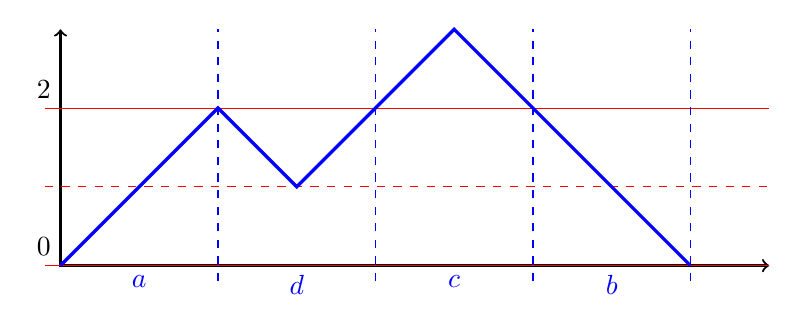
\begin{tikzpicture}
            \draw[<->, thick] (0, 3) -- (0, 0) -- (9, 0);
            \draw[dashed, red] (-.2, 1) --(9, 1);
            \draw[red] (-.2, 2) --(9, 2);
            \draw[red] (-.2, 0) --(9, 0);
            \draw[very thick, blue] (0, 0) -- (2, 2) -- (3, 1) -- (5, 3) -- (8, 0);
            \draw[blue, dashed] (2, -.2) -- (2, 3);
            \draw[blue, dashed] (4, -.2) -- (4, 3);
            \draw[blue, dashed] (6, -.2) -- (6, 3);
            \draw[blue, dashed] (8, -.2) -- (8, 3);
            \draw[blue] (1, 0) node[below] {$a$};
            \draw[blue] (3, 0) node[below] {$d$};
            \draw[blue] (5, 0) node[below] {$c$};
            \draw[blue] (7, 0) node[below] {$b$};
            \draw (0, 2) node[above left] {2};
            \draw (0, 0) node[above left] {0};
        \end{tikzpicture}
        \caption{Illustration of the letters of $\mathcal{A}$ using Dyck's representation.}
        \label{tikz:dyck2alphabet}
    \end{figure}

    This property is important as it implies that every $\pm 3$ strings uses at least two letters.
    So by checking if a pair of letter as a substring of a word make it not a Dyck word, $\mathcal{A}^2$
    can be split into two sets described in \autoref{tab:partitionDyck2}.

    \begin{table}[htb]
        \centering
        \caption{Partition of $\mathcal{A}$ into $\mathcal{X}, \mathcal{V}$.}
        \label{tab:partitionDyck2}
        \begin{tabular}{|c|c|}
            \hline
            $\mathcal{X}$ & $aa$ $ac$ $bb$ $bd$ $cb$ $cd$ $da$ $dc$ \\
            \hline
            $\mathcal{V}$ & $ab$ $ad$ $ba$ $bc$ $ca$ $cc$ $db$ $dd$ \\
            \hline
        \end{tabular}


        \newpage
    \end{table}
    \begin{itemize}
        \item The set $\mathcal{X}$. First, every couple of letter which contains
              a $\pm 3$ strings is in $\mathcal{X}$. This first condition explains the belonging
              of $aa, ac, dc, da, cb, bb, bd, \textrm{and}\ cd $. Next, $cd$ and $dc$ belong
              to $\mathcal{X}$ because of the following property: For any valid Dyck word of
              height at most 2, the current height is bounded between 0 and 2, moreover after each
              letter the current height is even so both couple $cd$ and $dc$ start
              and finish on the same bound. Futhermore,  $cd$ and $dc$ are going
              above and below the height at which they start so both are going outside off the
              bounds, thus a word which contains $cd$ or $dc$ can not be a Dyck Word of height a most 2.
              The \autoref{fig:rejectDyck2} shows each couple of $\mathcal{X}$.

              \begin{figure}[h!]
                  \centering
                  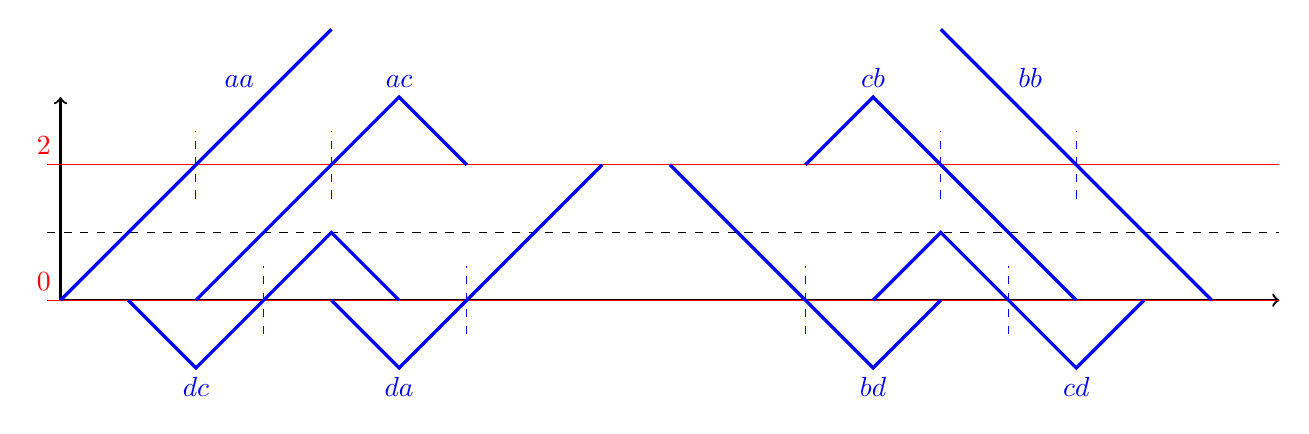
\begin{tikzpicture}[scale=.86]
                      \draw[<->, thick] (0, 3) -- (0, 0) -- (18, 0);
                      \draw[dashed] (-.2, 1) --(18, 1);
                      \draw[red] (-.2, 2) --(18, 2);
                      \draw[red] (-.2, 0) --(18, 0);
                      \draw[blue, very thick] (0, 0) -- (4, 4);
                      \draw[blue, very thick] (1, 0) -- (2, -1) -- (4, 1) -- (5, 0);
                      \draw[blue, very thick] (2,0) -- (5, 3) -- (6, 2);
                      \draw[blue, very thick] (4, 0) -- (5, -1) -- (8, 2);
                      \draw[blue, very thick] (9, 2) -- (12, -1) -- (13, 0);
                      \draw[blue, very thick] (12, 0) -- (13, 1) -- (15, -1) -- (16, 0);
                      \draw[blue, very thick] (11, 2) -- (12, 3) -- (15, 0);
                      \draw[blue, very thick] (13, 4)--(17,0);
                      \draw[red] (0, 2) node[above left] {2};
                      \draw[red] (0, 0) node[above left] {0};
                      \draw[blue] (2, -1) node[below] {$dc$};
                      \draw[blue] (5, -1) node[below] {$da$};
                      \draw[blue] (12, -1) node[below] {$bd$};
                      \draw[blue] (15, -1) node[below] {$cd$};
                      \draw[blue] (3, 3) node[above left] {$aa$};
                      \draw[blue] (5, 3) node[above] {$ac$};
                      \draw[blue] (12, 3) node[above] {$cb$};
                      \draw[blue] (14, 3) node[above right] {$bb$};
                      \draw[blue, dashed] (2, 2-.5) -- (2, 2.5);
                      \draw[blue, dashed] (3, -.5) -- (3, .5);
                      \draw[blue, dashed] (6, -.5) -- (6, .5);
                      \draw[blue, dashed] (4, 2-.5) -- (4, 2.5);
                      \draw[blue, dashed] (3, -.5) -- (3, .5);
                      \draw[blue, dashed] (11, -.5) -- (11, .5);
                      \draw[blue, dashed] (13, 2-.5) -- (13, 2.5);
                      \draw[blue, dashed] (14, -.5) -- (14, .5);
                      \draw[blue, dashed] (15, 1.5) -- (15, 2.5);
                  \end{tikzpicture}
                  \caption{Every 2 letters configuration that implies the word, whom
                      the configuration is a substring, is not a Dyck word of height at most 2.}
                  \label{fig:rejectDyck2}
              \end{figure}

        \item The set $\mathcal{V}$. The couples of $\mathcal{A}$ do not imply
              that the word is not a Dyck word of height at most 2 because each couple
              can fit inside the height bounds. The \autoref{fig:donotrejectDyck2} shows that
              every couple not in $\mathcal{X}$ (ie. $ab, ad, ba, bc, ca, cc, db, dd$)
              fit between height 0 and 2.



              \begin{figure}[h!]
                  \centering
                  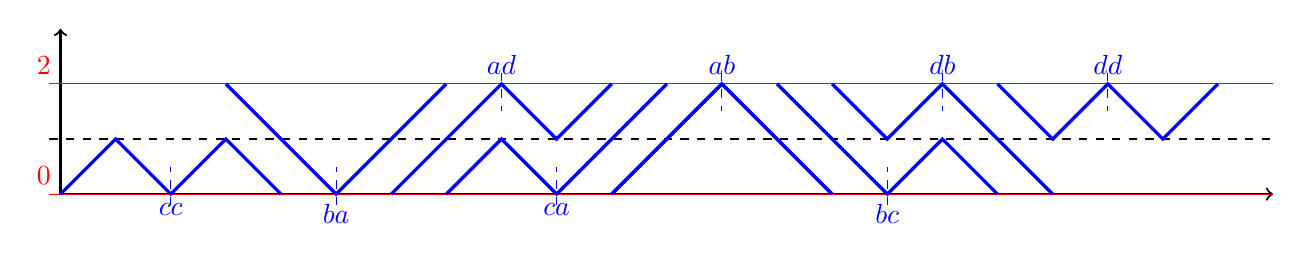
\begin{tikzpicture}[scale=.7]
                      \draw[<->, thick] (0, 3) -- (0, 0) -- (22, 0);
                      \draw[dashed] (-.2, 1) --(22, 1);
                      \draw[red] (-.2, 2) --(22, 2);
                      \draw[red] (-.2, 0) --(22, 0);
                      \draw[red] (0, 2) node[above left] {2};
                      \draw[red] (0, 0) node[above left] {0};
                      \draw[blue, very thick] (10, 0) -- (12, 2) -- (14, 0);
                      \draw[blue, very thick] (13, 2) -- (15, 0) -- (16, 1) -- (17, 0);
                      \draw[blue, very thick] (14, 2) -- (15, 1) -- (16, 2) -- (18, 0);
                      \draw[very thick, blue] (17 ,2) -- (18, 1) -- (19, 2) -- (20, 1) -- (21, 2);
                      \draw[blue, very thick] (10, 0) -- (12, 2) -- (14, 0);
                      \draw[blue, very thick] (11, 2) -- (9, 0) -- (8, 1) -- (7, 0);
                      \draw[blue, very thick] (10, 2) -- (9, 1) -- (8, 2) -- (6, 0);
                      \draw[blue, very thick] (7, 2) -- (5, 0) -- (3, 2);
                      \draw[very thick, blue] (4 ,0) -- (3, 1) -- (2, 0) -- (1, 1) -- (0, 0);
                      \draw[blue] (2, 0) node[below] {$cc$};
                      \draw[blue] (5, 0) node[below] {$ba$};
                      \draw[blue] (8, 2) node[above] {$ad$};
                      \draw[blue] (9, 0) node[below] {$ca$};
                      \draw[blue] (12, 2) node[above] {$ab$};
                      \draw[blue] (15, 0) node[below] {$bc$};
                      \draw[blue] (16, 2) node[above] {$db$};
                      \draw[blue] (19, 2) node[above] {$dd$};
                      \draw[blue, dashed] (2,-.2) -- (2, .5);
                      \draw[blue, dashed] (5, -.2) -- (5, .5);
                      \draw[blue, dashed] (9, -.2) -- (9, .5);
                      \draw[blue, dashed] (8, 2.2) -- (8, 1.5);
                      \draw[blue, dashed] (12, 2.2) -- (12, 1.5);
                      \draw[blue, dashed] (16, 2.2) -- (16, 1.5);
                      \draw[blue, dashed] (19, 2.2) -- (19, 1.5);
                      \draw[blue, dashed] (15, -.2) -- (15, .5);
                  \end{tikzpicture}
                  \caption{Every 2 letters configuration that
                      can be found in a valid Dyck word of height at most 2.}
                  \label{fig:donotrejectDyck2}
              \end{figure}
    \end{itemize}

    So a word, whose letter representation has a substring in $\mathcal{X}$,
    cannot be a Dyck word of height two. But does every non Dyck word of height
    at most 2 have a substring in $\mathcal{X}$?

    A word is not a dyck word of height at most 2 if it include a $\pm 3$ strings.
    But how are represented $\pm 3$ strings using the letters? There are 8
    different cases which are 2 by 2 symmetrical so \autoref{fig:p3string}
    and \autoref{fig:p3string2piece} show only the cases for +3 strings. In
    \autoref{fig:p3string}, every +3 string of size 3 is include in $aa$ or
    $ac$ so it is sufficient to search for this two couple. In \autoref{fig:p3string2piece}
    every +3 strings of length greater than 3 are composed of 2 minimal +2
    strings. This implies that one must be a $a$ while the other must be $da$
    of $dc$. Because $da$ or $dc$ are rejecting substrings, it is sufficient
    to search for them.

    \begin{figure}[h!]
        \begin{minipage}{.35\textwidth}
            \centering
            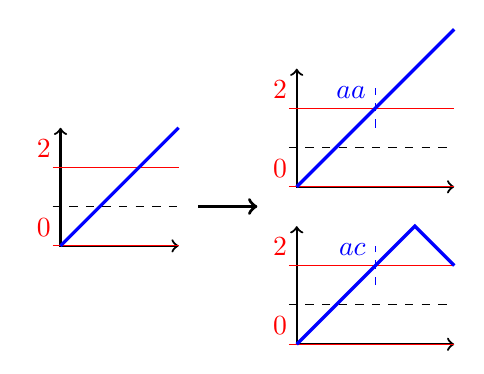
\begin{tikzpicture}[scale=.5]
                \draw[<->, thick] (0, 3) -- (0, 0) -- (3, 0);
                \draw[dashed] (-.2, 1) --(3, 1);
                \draw[red] (-.2, 2) --(3, 2);
                \draw[red] (-.2, 0) --(3, 0);
                \draw[red] (0, 2) node[above left] {2};
                \draw[red] (0, 0) node[above left] {0};
                \draw[blue, very thick] (0, 0) -- (3, 3);
                \draw[->, very thick] (3.5, 1) -- (5, 1);

                \draw[<->, thick] (6, 4+.5) -- (6, 1+.5) -- (10, 1+.5);
                \draw[dashed] (5.8,2+.5) -- (10,2+.5);
                \draw[red] (5.8,3+.5) -- (10,3+.5);
                \draw[red] (5.8,1+.5) -- (10, 1+.5);
                \draw[red] (6, 3+.5) node[above left] {2};
                \draw[red] (6, 1+.5) node[above left] {0};
                \draw[blue, very thick] (6, 1+.5) -- (10, 5+.5);
                \draw[blue, dashed] (8, 2.5+.5) -- (8, 3.5+.5);
                \draw[blue] (8, 3+.5) node[above left] {$aa$};

                \draw[<->, thick] (6, 4-4+.5) -- (6, 1-4+.5) -- (10, 1-4+.5);
                \draw[dashed] (5.8,2-4+.5) -- (10,2-4+.5);
                \draw[red] (5.8,3-4+.5) -- (10,3-4+.5);
                \draw[red] (5.8,1-4+.5) -- (10, 1-4+.5);
                \draw[red] (6, 3-4+.5) node[above left] {2};
                \draw[red] (6, 1-4+.5) node[above left] {0};
                \draw[blue, very thick] (6, 1-4+.5) -- (9, 0+.5) -- (10, -1+.5);
                \draw[blue, dashed] (8, 2.5-4+.5) -- (8, 3.5-4+.5);
                \draw[blue] (8, 3-4+.5) node[above left] {$ac$};
            \end{tikzpicture}
            \caption{Configuration for a +3 strings of size 3.}
            \label{fig:p3string}
        \end{minipage}
        \hfill
        \begin{minipage}{.60\textwidth}
            \centering
            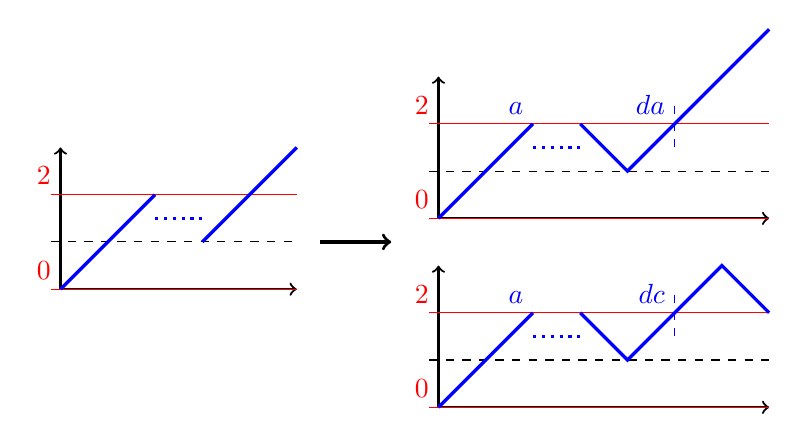
\begin{tikzpicture}[scale=.6]
                \draw[<->, thick] (0, 3) -- (0, 0) -- (5, 0);
                \draw[dashed] (-.2, 1) --(5, 1);
                \draw[red] (-.2, 2) --(5, 2);
                \draw[red] (-.2, 0) --(5, 0);
                \draw[red] (0, 2) node[above left] {2};
                \draw[red] (0, 0) node[above left] {0};
                \draw[blue, very thick] (0, 0) -- (2, 2);
                \draw[blue, very thick, dotted] (2, 1.5) -- (3, 1.5);
                \draw[blue, very thick] (3, 1) -- (5, 3);
                \draw[->, very thick] (5.5, 1) -- (7, 1);

                \draw[<->, thick] (8+0, 3+1.5) -- (8+0, 0+1.5) -- (8+5+2, 0+1.5);
                \draw[dashed] (8+-.2, 1+1.5) --(8+5+2, 1+1.5);
                \draw[red] (8+-.2, 2+1.5) --(8+5+2, 2+1.5);
                \draw[red] (8+-.2, 0+1.5) --(8+5+2, 0+1.5);
                \draw[red] (8+0, 2+1.5) node[above left] {2};
                \draw[red] (8+0, 0+1.5) node[above left] {0};
                \draw[blue, very thick] (8+0, 0+1.5) -- (8+2, 2+1.5);
                \draw[blue, very thick, dotted] (8+2, 1.5+1.5) -- (8+3, 1.5+1.5);
                \draw[blue, very thick] (8+3, 2+1.5) -- (8+4, 1+1.5) -- (8+7, 4+1.5);
                \draw[blue, dashed] (13, 1.5+1.5) -- (13, 4);
                \draw[blue] (13, -.5+4) node[above left] {$da$};
                \draw[blue] (10, -.5+4) node[above left] {$a$};

                \draw[<->, thick] (8+0, 3+1.5-4) -- (8+0, 0+1.5-4) -- (8+5+2, 0+1.5-4);
                \draw[dashed] (8+-.2, 1+1.5-4) --(8+5+2, 1+1.5-4);
                \draw[red] (8+-.2, 2+1.5-4) --(8+5+2, 2+1.5-4);
                \draw[red] (8+-.2, 0+1.5-4) --(8+5+2, 0+1.5-4);
                \draw[red] (8+0, 2+1.5-4) node[above left] {2};
                \draw[red] (8+0, 0+1.5-4) node[above left] {0};
                \draw[blue, very thick] (8+0, 0+1.5-4) -- (8+2, 2+1.5-4);
                \draw[blue, very thick, dotted] (8+2, 1.5+1.5-4) -- (8+3, 1.5+1.5-4);
                \draw[blue, very thick] (8+3, 2+1.5-4) -- (8+4, 1+1.5-4) -- (8+6, 3+1.5-4) -- (8+7, 2+1.5-4);
                \draw[blue, dashed] (13, -1) -- (13, 0);
                \draw[blue] (13, -.5) node[above left] {$dc$};
                \draw[blue] (10, -.5) node[above left] {$a$};

            \end{tikzpicture}
            \caption{Configurations for a +3 string of size greater than 3.}
            \label{fig:p3string2piece}
        \end{minipage}
    \end{figure}

\end{tproof}
Finally, a word on the alphabet $\mathcal{A}$ embodies a Dyck word of
height at most 2 if and only if it does not contain $aa, ac, bb, bd, cb, cd, da, dc$
as substrings. The following \textsc{Algorithm} \autoref{alg:dyck2nsqrt} for \Dyck{2, n}
comes from the direct application of the theorem.


\begin{algorithm}
    \caption{\textsc{DyckFast}$_{2,n}$}\label{alg:dyck2nsqrt}
    \begin{algorithmic}
        \Require $n \geq 0$, $x$ such that  $|x| = 2n$
        \State $x \gets 11x00$
        \State $\texttt{t} \gets \Null$
        \For{$\texttt{reject\_symbol} \in \{aa, ac, bb, bd, cb, cd, da, dc\}$}
        \If{$t == \Null$}
        \State \textbf{Find} $\texttt{t}$ in $\llbracket0, n\rrbracket$ such that \\
        \hspace*{1cm} $x[2\texttt{t}, \ldots, 2\texttt{t}+3] = \texttt{reject\_symbol}$
        \EndIf
        \EndFor
        \State \textbf{return} $\texttt{t} == \Null$

    \end{algorithmic}
\end{algorithm}

\begin{theorem}{\textbf{The quantum query complexity of \textsc{DyckFast}$_{2,n}$.}}
    The \textsc{DyckFast}$_{2,n}$ algorithm has a quantum query complexity of $O\left(\sqrt{n}\right)$.
\end{theorem}

\begin{tproof}
    The algorithm is doing at most 8 Grover's search on the modified input string $11x00$.
    So the total quantum query complexity is the folling.
    \[Q(\textsc{DyckFast}_{2, n}) = 8\times O\left(\sqrt{n+4}\right) = O\left(\sqrt{n}\right)\]
\end{tproof}

\subsection{A new algorithm for k=3}

\subsection{A try for a new algorithm for any k.}
